\documentclass[10pt, letterpaper, answer]{exam}
\usepackage{graphicx, amsmath, tikz}   
\usepackage[margin=1in]{geometry}
\usetikzlibrary{decorations.pathreplacing} 

% Comment this out to remove answer boxes.
\printanswers

\newcommand*{\TickSize}{2pt}%

\newcommand*{\AxisMin}{0}%
\newcommand*{\AxisMax}{0}%


\title{Math 215: Bifurcation and hysteresis in the Energy Balance Model}

\author{Sven Bachmann, Nathan Bailey and Peter Harrington}

\date{}

\begin{document}
\maketitle

\section{The model}

The Energy Balance Model (EBM) describes the change of (average) global temperature on earth $T$ using a simple model of energy fluxes. It postulates that the rate of change in the Earth's temperature is proportional to the difference between the incoming and outgoing rates of energy transfer, the former one due to radiation from the sun and the latter one being radiated back by the earth's surface through the atmosphere. The EBM equation is given by
\begin{equation}\label{EBM}
    \dfrac{dT}{dt} = A(1 - \alpha(T)) - B\epsilon T^4.
\end{equation}
where the constants $A,B$ have value
\begin{equation}
    A = 1.7445 \times 10^{-6} Ks^{-1},\quad
    B = 2.8987 \times 10^{-16} K^{-3}s^{-1}.
\end{equation}
Here, the unitless function $\alpha(T) \in [0,1]$ is the \emph{albedo}, namely the proportion of light reflected off of the earth's surface, while the \emph{emissivity}  $\epsilon$ describes the fraction of energy radiated away from the surface of the earth that escapes out of the atmosphere.

The albedo is higher at low temperatures since sea ice reflects off more light than the dark oceans. A standard model for $\alpha(T)$ is given by


\begin{equation}
   \alpha (T)=0.7-0.4\frac{e^{(T-263)/4}}{1+e^{(T-263)/4}}. 
\end{equation}

\begin{center}
   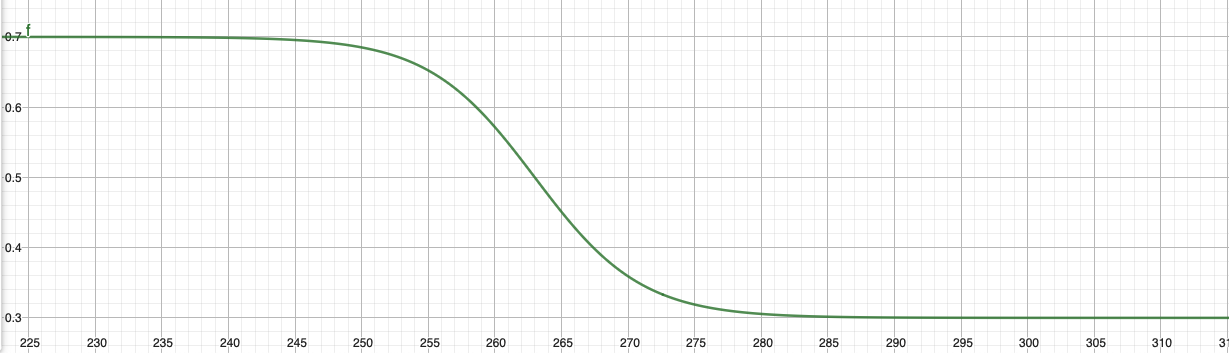
\includegraphics[width=0.75\textwidth]{Albedo.png} 
\end{center}

\bigskip



\newpage

\section{Questions}

\begin{enumerate}
\item In the graph below, we plot $1-\alpha(T)$ as well as $\frac{B}{A}\epsilon$ for various values of $\epsilon$:

\begin{figure}[!h]\begin{center}
    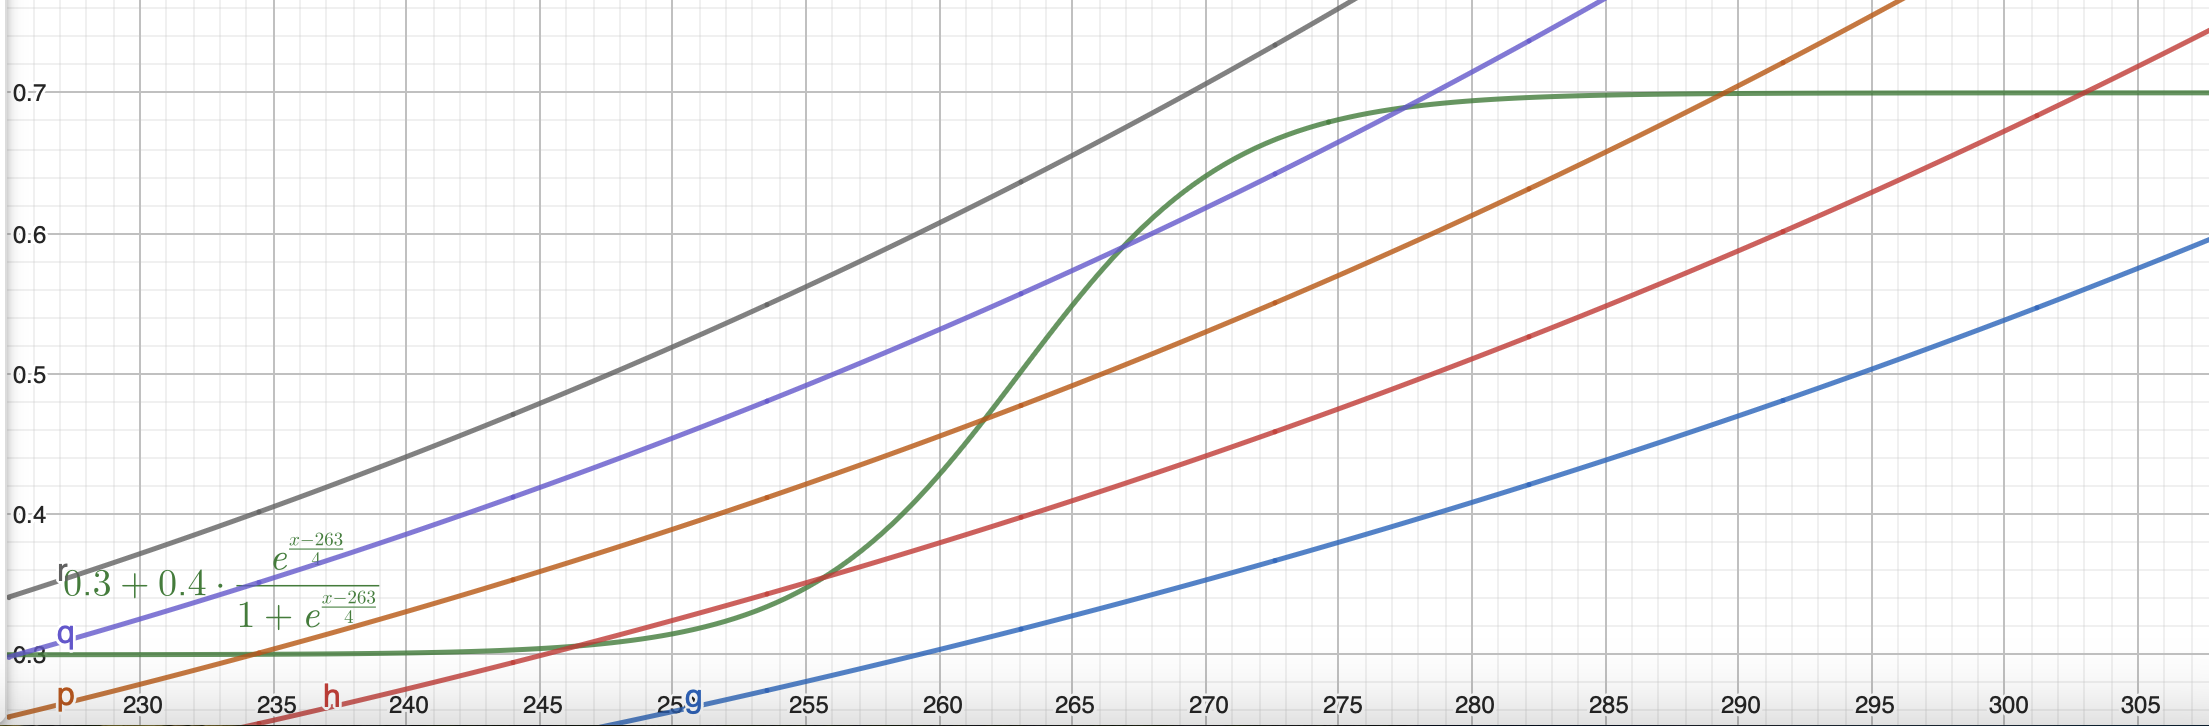
\includegraphics[width=0.75\textwidth]{Bifurcation.png}
    \caption{The thick black curve is $1-\alpha(T)$ while the coloured curves are $\frac{B}{A}\epsilon T^4$ for increasing values of $\epsilon$, with $\epsilon =0.4,0.5,0.6,0.7,0.8$ from bottom to top} 
\end{center}
\label{TheGraph}\end{figure} 

For each value of $\epsilon$ above, determine all critical points and their stability. Sketch the phase line. \\ \emph{Hint.} No calculation is needed, the graph above suffices. 






    
\item The function $A(1-\alpha(T))-B\epsilon T^4$ depends smoothly on the variables $(\epsilon,T)$ and hence so do its zeroes. Using the phase lines above, sketch a line of critical points in the $(\epsilon,T)$ plane, and label the stability of the critical points.


\item The current mean surface temperature being $14C\approx 287K$, estimate the emissivity $\epsilon$.

\item The emissivity is critically influenced by the greenhouse effect: An atmosphere with a higher concentration of greenhouse gases captures more energy and therefore corresponds to a lower emissivity. What effect on the mean global temperature does the model predict under such a decrease of emissivity?

\item Assume on the contrary that $\epsilon$ increases slowly from the current value to $0.8$. Describe the evolution of the mean temperature.

\item Continue from the previous solution and analyse the temperature's evolution as the emissivity now decreases from 0.8 to the current value $\epsilon = 0.62$.

 
\end{enumerate}

\newpage 

\section{More details}

\subsection{The physical model
}
The physically more complete form of the EBM expresses that the rate of temperature change is proportional to the difference of incoming and outgoing power (rate of energy transfer), which are expressed explicitly as

\begin{equation}
    C \frac{d T}{d t} = P_{\rm in} - P_{\rm out} = \pi r^2 Q (1-\alpha(T)) - 4 \pi r^2 \sigma \epsilon T^4.
\end{equation}
where $t$ is time (expressed in seconds) and 
\begin{center}
\begin{tabular}{ l | l | l }
Symbol & Definition & Units \\
\hline \hline
$T > 0$ & Mean global temperature of the Earth & $K$ \\
$P$ & Power & $W=J s^{-1}$ \\
$C$ & Heat capacity of the Earth & $J K^{-1}$\\  
$\alpha(T)$ & Albedo & unitless \\
$r$ & Earth radius & $m$ \\
$Q$ & Incoming energy density & $W m^{-2}$ \\
$\sigma$ & Stefan-Boltzmann constant & $Wm^{-2}K^{-4}$ \\
$\epsilon$ & emissivity & unitless
\end{tabular}
\end{center}

The parameter $Q$ represents the rate of incoming solar energy reaching the Earth per square meter and the constant $\sigma$ is a universal physical constant. The values of the constants are as follows: 
$$
\begin{cases}
    C & = 1.0 \times 10^{23} J K^{-1} \\
    r & = 6.3781 \times 10^{6}m \\
    Q & = 1365 W m^{-2} \\
    \sigma &= 5.6704 \times 10^{-8} W m^{-2} K^{-4}.
\end{cases}
$$

\subsection{Local bifurcation}

One phenomenon observed in this exercise is that of a bifurcation, where a stable equilibrium point ceases to exist as a parameter (here the emissivity) varies. This yields to an abrupt change in the equilibrium state of the system as the parameter smoothly crosses the critical value. While it is unclear if the earth was ever in the snowball state described in Question~5 above, the bifurcation analysis has been used `locally' on earth, with (a refinement of) the model discussed here discribing the polar regions of the planet.

Finally, we note that the phenomena of bifurcation and hysteresis observed above, appears in popular discussions on climate change under the name \emph{tipping point}.

\end{document}